% TargetCamera

\section{\class{TargetCamera} ---
         Target camera}

The \class{TargetCamera} class always looks at a specified point and
aligns its local up direction to the scene up direction.

\begin{classdesc}{TargetCamera}{name = "TargetCamera",\\ 
                       target = (0,0,0),\\
                       fov = 45.0,\\
                       roll = 0.0, \\
                       up = None,\\
                       focallength = 0,\\
                       fstop = 0,\\
                       auto_nearfar = True,\\
                       nearplane = 0.1,\\
                       farplane = 1000.0,\\
                       }

\var{target} is the point that the camera will always look at. 

\var{fov} is the field of view in degrees (in vertical direction), i.e.
the angle between the bottom and the top of the screen.

\var{roll} is an angle in degrees that the camera is rotated about its 
local z axis.

\var{up} is the vector that is considered to be the 'up' direction. If
\code{None} is passed, the global 'up' direction from the scene is used.

\var{focallength} is the focal length of the camera and \var{fstop} the
aperture number that determines the lens diameter. These values are used
to turn on depth of field. Depth of field is activated if both attributes
are set to a value different from 0 (note however, that not every renderer
supports depth of field). The focal distance is set so that the target 
point will always be in focus.

\var{auto_nearfar} specifies whether the near and far plane
distances are automatically determined or if fixed values are used.
If set to \code{False}, the \var{nearplane} and \var{farplane} arguments
are used, otherwise the values are computed from the objects in the scene.
In the latter case, the \var{nearplane} value still serves as minimum
value for the near plane distance which is used when the camera is located
within the scene bounds.
\end{classdesc}

The \class{TargetCamera} has the following slots (in addition to the slots
of the \class{WorldObject} base class):

\begin{tableiv}{l|l|c|l}{code}{Slot}{Type}{Access}{Description}
\lineiv{target_slot}{vec3}{rw}{Target point}
\lineiv{fov_slot}{float}{rw}{Field of view in degrees}
\lineiv{roll_slot}{float}{rw}{Rotation about local z axis (in degrees)}
\lineiv{up_slot}{vec3}{rw}{Up direction}
\lineiv{focallength_slot}{float}{rw}{Focal length of the camera}
\lineiv{fstop_slot}{float}{rw}{Aperture number}
\lineiv{autonearfar_slot}{bool}{rw}{Automatically compute near/far values?}
\lineiv{nearplane_slot}{float}{rw}{(Minimal) near plane distance}
\lineiv{farplane_slot}{float}{rw}{Far plane distance}
\end{tableiv}

\begin{methoddesc}{projection}{width, height, near, far}
Returns the projection matrix for a viewport with the given width and
height (actually only the ratio width/height is relevant). The near
and far clipping planes are set to \var{near} and \var{far}.
\end{methoddesc}

\begin{methoddesc}{viewTransformation}{}
Returns the view transformation for this camera.
\end{methoddesc}

\begin{methoddesc}{eyeRay}{x0, y0, width, height}
Return a ray whose origin is at the eye position and that goes through
a given point on the image plane. The point on the plane is given by
(\var{x0}, \var{y0}) which each ranges from 0 to 1. (0,0) is at the
upper left and (1,1) at the lower right corner. The arguments \var{width} and
\var{height} determine the ratio of the image plane (the absolute
values of \var{width} and
\var{height} are irrelevant). The return value is a 2-tuple (\var{p}, \var{u})
where \var{p} is the ray origin and \var{u} the normalized
direction. Both vectors are given in world space.

\begin{center}
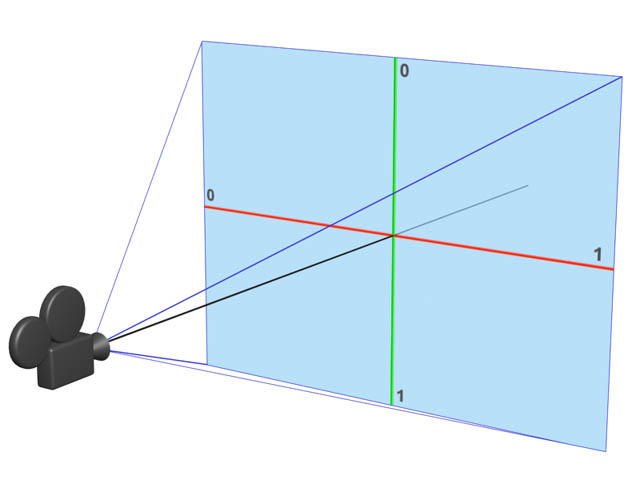
\includegraphics[width=9cm]{pics/camera01}
\end{center}
\end{methoddesc}

\begin{methoddesc}{getNearFar}{}
Return a 2-tuple (\var{near}, \var{far}) with the distances to the
near and far clipping planes. If automatic computation is disabled,
the method just returns the stored values, otherwise the values
are computed from the bounding box of the scene (which is converted
to a bounding sphere and the clipping planes are set as tangent planes
to the sphere).
\end{methoddesc}
